\documentclass[notes=show]{beamer}
%%%%%%%%%%%%%%%%%%%%%%%%%%%%%%%%%%%%%%%%%%%%%%%%%%%%%%%%%%%%%%%%%%%%%%%%%%%%%%%%%%%%%%%%%%%%%%%%%%%%%%%%%%%%%%%%%%%%%%%%%%%%%%%%%%%%%%%%%%%%%%%%%%%%%%%%%%%%%%%%%%%%%%%%%%%%%%%%%%%%%%%%%%%%%%%%%%%%%%%%%%%%%%%%%%%%%%%%%%%%%%%%%%%%%%%%%%%%%%%%%%%%%%%%%%%%
\AtBeginSubsection[
  {\frame<beamer>{\frametitle{Outline}   
    \tableofcontents[currentsection,currentsubsection]}}%
]%
{
  \frame<beamer>{ 
    \frametitle{Outline}   
    \tableofcontents[currentsection,currentsubsection]}
}
\usepackage{ulem}
\usepackage{pdflscape}
\setbeamertemplate{caption}{\insertcaption}
\usepackage{color,xcolor,ucs}
\usepackage{beamerthemesplit}
\usepackage{graphicx}
\usepackage{amsmath}
\usepackage[export]{adjustbox}
\usepackage{pdfpages} 
\definecolor{mintgreen}{rgb}{0.6, 1.0, 0.6}
\makeatletter
\@addtoreset{subfigure}{framenumber}% subfigure counter resets every frame
\makeatother
\newcommand*{\Scale}[2][4]{\scalebox{#1}{$#2$}}%
\newcommand*{\Resize}[2]{\resizebox{#1}{!}{$#2$}}%
\usepackage{amsfonts}
\usepackage{booktabs}
\usepackage{color,soul}
\usepackage{pdfpages}
\setboolean{@twoside}{false}
\usepackage{amsmath}
\usepackage{pdflscape} 
\usepackage{eurosym}
\usepackage{amstext} % for \text
\DeclareRobustCommand{\officialeuro}{%
  \ifmmode\expandafter\text\fi
  {\fontencoding{U}\fontfamily{eurosym}\selectfont e}}
\usepackage[caption = false]{subfig}
\usepackage{appendixnumberbeamer} 
\usepackage{graphicx}
\usepackage{mathpazo}
\usepackage{hyperref}
\usepackage{multimedia}
\usepackage{graphicx}
\usepackage{multirow}
\usepackage{subfig}
\usepackage{verbatim}
\usepackage{booktabs, multicol, multirow}
\setcounter{MaxMatrixCols}{10}
% Define new binary operators


%Comandi che riteniamo utili, presi da Abadir_Magnus.

% operatornames
\newcommand{\bias}{\operatorname{bias}}
\newcommand{\col}{\operatorname{col}}
\newcommand{\corr}{\operatorname{corr}}
\newcommand{\cov}{\operatorname{cov}}
\newcommand{\dg}{\operatorname{dg}}
\newcommand{\diag}{\operatorname{diag}}
\newcommand{\E}{\operatorname{E}}
\newcommand{\etr}{\operatorname{etr}}
\newcommand{\kur}{\operatorname{kur}}
%\newcommand{\median}{\operatorname{med}}
\newcommand{\MSE}{\operatorname{MSE}}
\newcommand{\plim}{\operatorname{plim}}
\newcommand{\rk}{\operatorname{rk}}
\newcommand{\sgn}{\operatorname{sgn}}
\newcommand{\tr}{\operatorname{tr}}
\newcommand{\var}{\operatorname{var}}
\renewcommand{\vec}{\operatorname{vec}}
\newcommand{\vech}{\operatorname{vech}}

\newcommand{\SC}{\mathbb{C}}
\newcommand{\SN}{\mathbb{N}}
\newcommand{\SQ}{\mathbb{Q}}
\newcommand{\SR}{\mathbb{R}}
\newcommand{\SZ}{\mathbb{Z}}
%
% calligraphic capital letters
\newcommand{\calA}{\mathcal{A}}
\newcommand{\calB}{\mathcal{B}}
\newcommand{\calC}{\mathcal{C}}
\newcommand{\calD}{\mathcal{D}}
\newcommand{\calE}{\mathcal{E}}
\newcommand{\calF}{\mathcal{F}}
\newcommand{\calG}{\mathcal{G}}
\newcommand{\calH}{\mathcal{H}}
\newcommand{\calI}{\mathcal{I}}
\newcommand{\calJ}{\mathcal{J}}
\newcommand{\calK}{\mathcal{K}}
\newcommand{\calL}{\mathcal{L}}
\newcommand{\calM}{\mathcal{M}}
\newcommand{\calN}{\mathcal{N}}
\newcommand{\calO}{\mathcal{O}}
\newcommand{\calP}{\mathcal{P}}
\newcommand{\calQ}{\mathcal{Q}}
\newcommand{\calR}{\mathcal{R}}
\newcommand{\calS}{\mathcal{S}}
\newcommand{\calT}{\mathcal{T}}
\newcommand{\calU}{\mathcal{U}}
\newcommand{\calV}{\mathcal{V}}
\newcommand{\calW}{\mathcal{W}}
\newcommand{\calX}{\mathcal{X}}
\newcommand{\calY}{\mathcal{Y}}
\newcommand{\calZ}{\mathcal{Z}}
%
% bold lowercase and capital letters for vectors (v) and matrices (m)
\newcommand{\mA}{\bm A}
\newcommand{\va}{\bm a}
\newcommand{\mB}{\bm B}
\newcommand{\vb}{\bm b}
\newcommand{\mC}{\bm C}
\newcommand{\vc}{\bm c}
\newcommand{\mD}{\bm D}
\newcommand{\vd}{\bm d}
\newcommand{\mE}{\bm E}
\newcommand{\ve}{\bm e}
\newcommand{\mF}{\bm F}
\newcommand{\vf}{\bm f}
\newcommand{\mG}{\bm G}
\newcommand{\vg}{\bm g}
\newcommand{\mH}{\bm H}
\newcommand{\vh}{\bm h}
\newcommand{\mI}{\bm I}
\newcommand{\vi}{\bm i}
\newcommand{\mJ}{\bm J}
\newcommand{\vj}{\bm j}
\newcommand{\mK}{\bm K}
\newcommand{\vk}{\bm k}
\newcommand{\mL}{\bm L}
\newcommand{\vl}{\bm l}
\newcommand{\mM}{\bm M}
\newcommand{\vm}{\bm m}
\newcommand{\mN}{\bm N}
\newcommand{\vn}{\bm n}
\newcommand{\mO}{\bm O}
\newcommand{\vo}{\bm o}
\newcommand{\mP}{\bm P}
\newcommand{\vp}{\bm p}
\newcommand{\mQ}{\bm Q}
\newcommand{\vq}{\bm q}
\newcommand{\mR}{\bm R}
\newcommand{\vr}{\bm r}
\newcommand{\mS}{\bm S}
\newcommand{\vs}{\bm s}
\newcommand{\mT}{\bm T}
\newcommand{\vt}{\bm t}
\newcommand{\mU}{\bm U}
\newcommand{\vu}{\bm u}
\newcommand{\mV}{\bm V}
\newcommand{\vv}{\bm v}
\newcommand{\mW}{\bm W}
\newcommand{\vw}{\bm w}
\newcommand{\mX}{\bm X}
\newcommand{\vx}{\bm x}
\newcommand{\mY}{\bm Y}
\newcommand{\vy}{\bm y}
\newcommand{\mZ}{\bm Z}
\newcommand{\vz}{\bm z}
%
% bold Greek lowercase letters for vectors (v)
\newcommand{\valpha}{\bm \alpha}
\newcommand{\vbeta}{\bm \beta}
\newcommand{\vgamma}{\bm \gamma}
\newcommand{\vdelta}{\bm \delta}
\newcommand{\vepsi}{\bm \epsi}
\newcommand{\vvarepsilon}{\bm \varepsilon}
\newcommand{\vzeta}{\bm \zeta}
\newcommand{\veta}{\bm \eta}
\newcommand{\vtheta}{\bm \theta}
\newcommand{\viota}{\bm \iota}
\newcommand{\vkappa}{\bm \kappa}
\newcommand{\vlambda}{\bm \lambda}
\newcommand{\vmu}{\bm \mu}
\newcommand{\vnu}{\bm \nu}
\newcommand{\vxi}{\bm \xi}
\newcommand{\vpi}{\bm \pi}
\newcommand{\vrho}{\bm \rho}
\newcommand{\vsigma}{\bm \sigma}
\newcommand{\vtau}{\bm \tau}
\newcommand{\vupsilon}{\bm \upsilon}
\newcommand{\vphi}{\bm \phi}
\newcommand{\vchi}{\bm \chi}
\newcommand{\vpsi}{\bm \psi}
\newcommand{\vomega}{\bm \omega}
%
% bold Greek capital letters for matrices (m)
\newcommand{\mGamma}{\bm \Gamma}
\newcommand{\mDelta}{\bm \varDelta}
\newcommand{\mTheta}{\bm \varTheta}
\newcommand{\mLambda}{\bm \varLambda}
\newcommand{\mXi}{\bm \varXi}
\newcommand{\mPi}{\bm \varPi}
\newcommand{\mSigma}{\bm \varSigma}
\newcommand{\mUpsilon}{\bm \varUpsilon}
\newcommand{\mPhi}{\bm \varPhi}
\newcommand{\mPsi}{\bm \varPsi}
\newcommand{\mOmega}{\bm \varOmega}


%Per i limiti
\newcommand{\longto}{\longrightarrow}
\newcommand{\pto}{\stackrel{p}{\longrightarrow}}
\newcommand{\dto}{\stackrel{d}{\longrightarrow}}
\newcommand{\wto}{\stackrel{w}{\longrightarrow}}

\def\convas{\mathbin{\buildrel{\rm as}\over\rightarrow}}
% \def\convd{\mathbin{\buildrel{\rm d}\over\rightarrow}}
\def\convd{\mathbin{\Rightarrow}}
\def\convms{\mathbin{\buildrel{\rm ms}\over\rightarrow}}
\def\convp{\mathbin{\buildrel{\rm p}\over\rightarrow}}
\def\convr{\mathbin{\buildrel{r{\rm th}}\over\rightarrow}}
\def\convs{\mathbin{\buildrel{s{\rm th}}\over\rightarrow}}

% Abbreviated commands (FP+RS)

\newcommand {\nn}{\nonumber}
\newcommand{\ba}{\begin{eqnarray}}
\newcommand{\be}{\begin{equation}}
\newcommand{\ban}{\begin{eqnarray*}}
\newcommand{\ea}{\end{eqnarray}}
\newcommand{\ean}{\end{eqnarray*}}
\newcommand{\ee}{\end{equation}}
\newcommand{\bw}{\hat{\beta}}
\newcommand{\smn}{\dfrac{1}{n}\sum_{i=1}^{n}}
\newcommand{\gammah}{\hat{\gamma}_{iT}}
\newcommand{\psih}{\hat{\psi}_{iT}}
\newcommand{\asy}{as $n\stackrel{}{\rightarrow} \infty$ with $T$ fixed}
\newcommand{\asyy}{$n\stackrel{}{\rightarrow} \infty$ with $T$ fixed}
\newcommand{\frecciap}{\stackrel{p}{\rightarrow}}
\newcommand{\freccia}{\stackrel{}{\rightarrow}}
\newcommand{\bws}{\hat{\beta}_{w,b,a}}
\newcommand{\borr}{\hat{\beta}_{orr}}
% Define new mathematical operators (fP)
\def\1{\mathop{1_{}}\nolimits}
\def\AMSE{\mathop{\rm AMSE}\nolimits}
\def\AR{\mathop{\rm AR}\nolimits}
\def\ARCH{\mathop{\rm ARCH}\nolimits}
\def\ARE{\mathop{\rm ARE}\nolimits}
\def\ARIMA{\mathop{\rm ARIMA}\nolimits}
\def\ARMA{\mathop{\rm ARMA}\nolimits}
\def\argmax{\mathop{\rm argmax}}
\def\argmin{\mathop{\rm argmin}}
\def\AVh{\mathop{\widehat{\rm AV}}\nolimits}
\def\AV{\mathop{\rm AV}\nolimits}
\def\Bias{\mathop{\rm Bias}\nolimits}
\def\Biash{\mathop{\widehat{\rm Bias}}\nolimits}
\def\Biast{\mathop{{\rm Bias}_\theta}\nolimits}
\def\CI{\mathop{\rm CI}\nolimits}
\def\Corr{\mathop{\rm Corr}\nolimits}
\def\Cov{\mathop{\rm Cov}\nolimits}
\def\CovF{\mathop{{\rm Cov}_F}\nolimits}
\def\CovFh{\mathop{{\rm Cov}_{\hat{F}}}\nolimits}
\def\Covh{\mathop{\widehat{\rm Cov}}\nolimits}
\def\Covt{\mathop{{\rm Cov}_\theta}\nolimits}
\def\diag{\mathop{{\rm diag}}\nolimits}
\def\CV{\mathop{\rm CV}\nolimits}
\def\dh{\hat\delta}
\def\E{\mathop{{\rm E}_{}}\nolimits}
\def\EIF{\mathop{\rm EIF}\nolimits}
\def\Et{\mathop{{\rm E}_\theta}\nolimits}
\def\EF{\mathop{{\rm E}_F}\nolimits}
\def\EFh{\mathop{{\rm E}_{\hat{F}}}\nolimits}
\def\EFn{\mathop{{\rm E}_{F_n}}\nolimits}
\def\Eo{\mathop{{\rm E}_0}\nolimits}
\def\Et{\mathop{{\rm E}_\theta}\nolimits}
\def\GARCH{\mathop{\rm GARCH}\nolimits}
\def\IF{\mathop{\rm IF}\nolimits}
\def\MA{\mathop{\rm MA}\nolimits}
\def\MAD{\mathop{\rm MAD}\nolimits}
\def\Med{\mathop{\rm Med}\nolimits}
\def\MISE{\mathop{\rm MISE}\nolimits}
\def\MSD{\mathop{\rm MSD}\nolimits}
\def\MSE{\mathop{\rm MSE}\nolimits}
\def\MSEt{\mathop{{\rm MSE}_\theta}\nolimits}
\def\plim{\mathop{{\rm plim}_{}}\nolimits}
\def\PrF{\mathop{\Pr\nolimits_{F}}}
\def\PrFh{\mathop{\Pr\nolimits_{\hat{F}}}}
\def\Prh{\mathop{\widehat{\Pr}}\nolimits}
\def\Prt{\mathop{\Pr\nolimits_\theta}}
\def\rank{\mathop{\rm rank}\nolimits}
\def\SE{\mathop{\rm SE}\nolimits}
\def\SEh{\mathop{\widehat{\rm SE}}\nolimits}
\def\sign{\mathop{\rm sign}\nolimits}
\def\tan{\mathop{\rm tan}\nolimits}
\def\th{\hat\theta}
\def\trace{\mathop{\rm tr}\nolimits}
\def\Var{\mathop{\rm Var}\nolimits}
\def\VarF{\mathop{{\rm Var}_F}\nolimits}
\def\Varh{\mathop{\widehat{\rm Var}}\nolimits}
\def\VarFh{\mathop{{\rm Var}_{\hat{F}}}\nolimits}
\def\Vart{\mathop{{\rm Var}_\theta}\nolimits}
\def\WN{\mathop{\rm WN}\nolimits}

% Redefined LATEX commands

\renewcommand{\Im}{I_{m}}
% \Im redefines command for script I
\renewcommand{\mid}{\,|\,}
\renewcommand{\theenumii}{\theenumi.\arabic{enumii}}
% \renewcommand{\tt}{\tilde\theta}
\renewcommand{\to}{\theta_{0}}
\renewcommand{\u}{{\bf u}}
\renewcommand{\vec}{{\rm vec}\,}
\renewcommand{\Xi}{X_{i}}
% \Xi redefines command for upper-case xi
\AtBeginSection[]
{
  \begin{frame}[noframenumbering]
    \frametitle{Outline for section \thesection}
    \tableofcontents[currentsection]
  \end{frame}
}


\usepackage{xcolor,soul}
\renewcommand<>{\hl}[1]{\only#2{\beameroriginal{\hl}}{#1}}

% https://tex.stackexchange.com/questions/41683/why-is-it-that-coloring-in-soul-in-beamer-is-not-visible
\makeatletter
\newcommand\SoulColor{%
  \let\set@color\beamerorig@set@color
  \let\reset@color\beamerorig@reset@color}
\makeatother
\SoulColor
\AtBeginSection{\frame{\sectionpage}}

\newsavebox\mybox
\newenvironment{aquote}[1]
  {\savebox\mybox{#1}\begin{quote}\openautoquote\hspace*{-.7ex}}
  {\unskip\closeautoquote\vspace*{1mm}\signed{\usebox\mybox}\end{quote}}

\newtheorem{proposition}[theorem]{Proposition}
\newtheorem{Assumption}[theorem]{Assumption}
\newenvironment{stepenumerate}{\begin{enumerate}[<+->]}{\end{enumerate}}
\newenvironment{stepitemize}{\begin{itemize}[<+->]}{\end{itemize} }
\newenvironment{stepenumeratewithalert}{\begin{enumerate}[<+-| alert@+>]}{\end{enumerate}}
\newenvironment{stepitemizewithalert}{\begin{itemize}[<+-| alert@+>]}{\end{itemize} }
\usetheme{Madrid}
\makeatletter
\setbeamertemplate{footline}
{
  \leavevmode%
  \hbox{%
  \begin{beamercolorbox}[wd=.333333\paperwidth,ht=2.25ex,dp=1ex,center]{author in head/foot}%
    \usebeamerfont{author in head/foot}\insertshortauthor~~\beamer@ifempty{\insertshortinstitute}{}{(\insertshortinstitute)}
  \end{beamercolorbox}%
  \begin{beamercolorbox}[wd=.333333\paperwidth,ht=2.25ex,dp=1ex,center]{title in head/foot}%
    \usebeamerfont{title in head/foot}\insertshorttitle
  \end{beamercolorbox}%
  \begin{beamercolorbox}[wd=.333333\paperwidth,ht=2.25ex,dp=1ex,right]{date in head/foot}%
    \usebeamerfont{date in head/foot}\insertshortdate{}\hspace*{2em}
%    \insertframenumber{} / \inserttotalframenumber\hspace*{2ex} % DELETED
  \end{beamercolorbox}}%
  \vskip0pt%
}
\makeatother
\usepackage{pdfpages}
\begin{document}
	\title[]{\large Intro to Applied Econometrics Econ 628 / 2nd Half	\vspace{0.5cm}
	}
	\author[Raffaele Saggio - Econ 628]{Raffaele Saggio}
	\institute[]{UBC}
	\date{\today \\
}
	\maketitle

%%%%%%%%%%%%%%%%%%%%%%%%%	
%%%%%%%%%%%%%%%%%%%%%%%%%
%%%%%%%%%%%%%%%%%%%%%%%%%
%%%%%%%%%%%%%%%%%%%%%%%%%
\setbeamertemplate{footline}[frame number]{}

%gets rid of bottom navigation symbols
\setbeamertemplate{navigation symbols}{}

%gets rid of footer
%will override 'frame number' instruction above
%comment out to revert to previous/default definitions
\setbeamertemplate{footline}{}
%%
\begin{frame}
\frametitle{Why is this course important?}
\begin{figure}[htb]
\centering

\includegraphics[width=1\textwidth]{kleven0}
\end{figure}
\end{frame}
\begin{frame}
\frametitle{Why is this course important?}
\begin{figure}[htb]
\centering
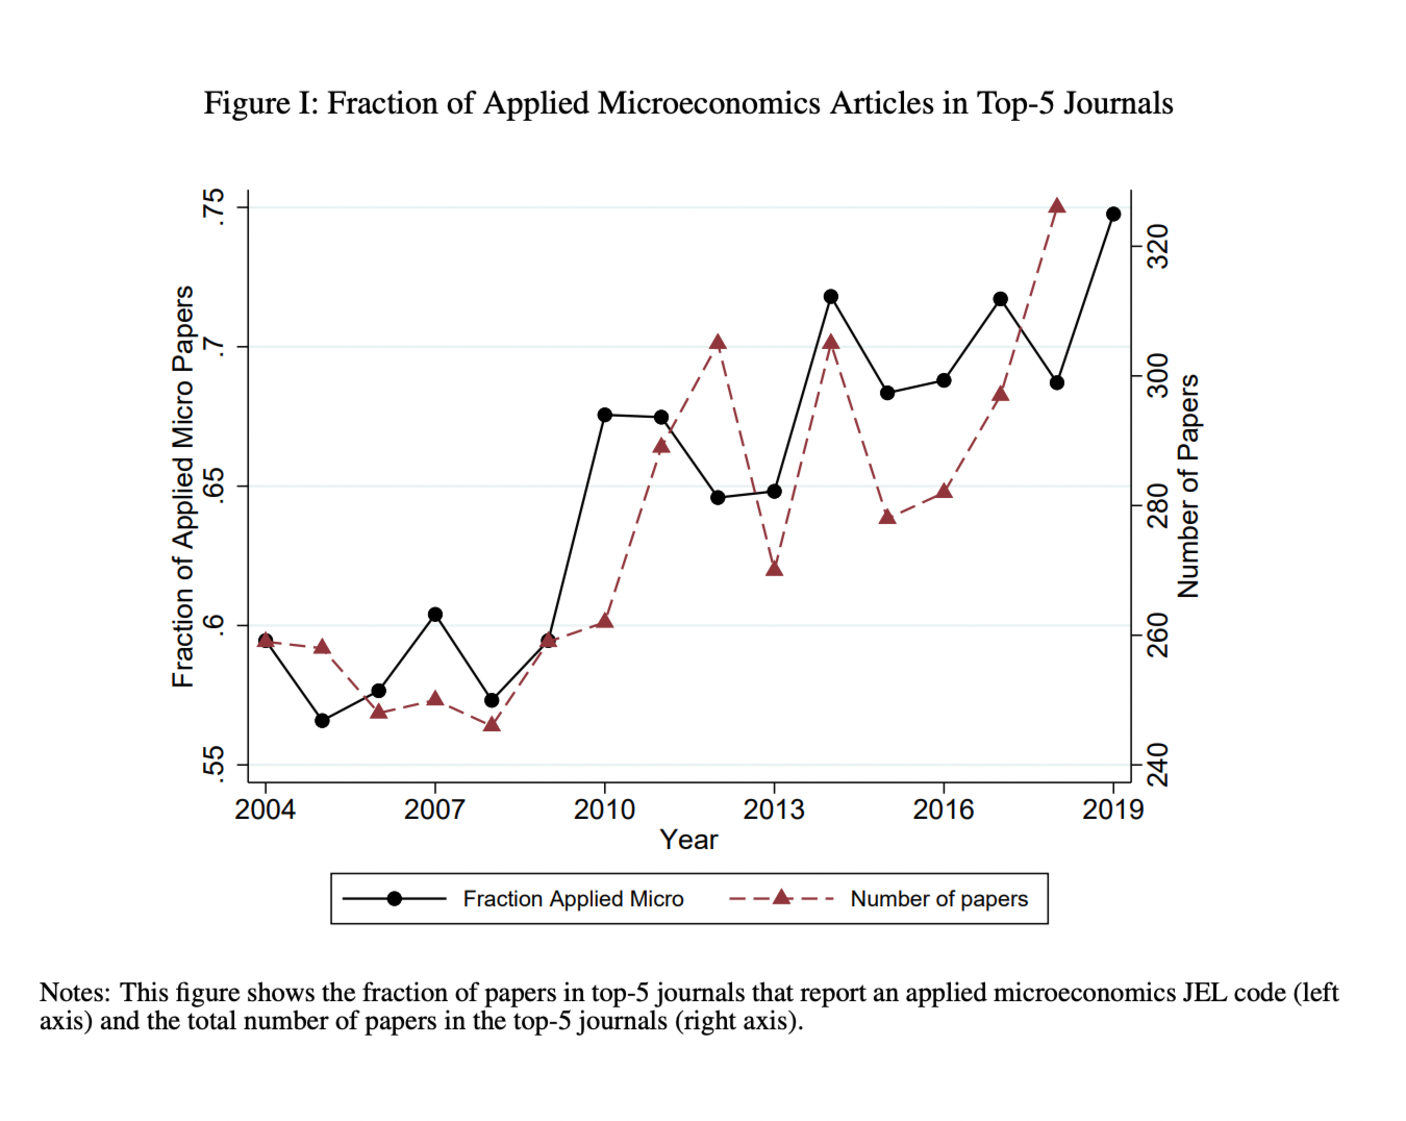
\includegraphics[width=1\textwidth]{kleven1}
\end{figure}
\end{frame}
\begin{frame}
\frametitle{Why is this course important?}
\begin{figure}[htb]
\centering
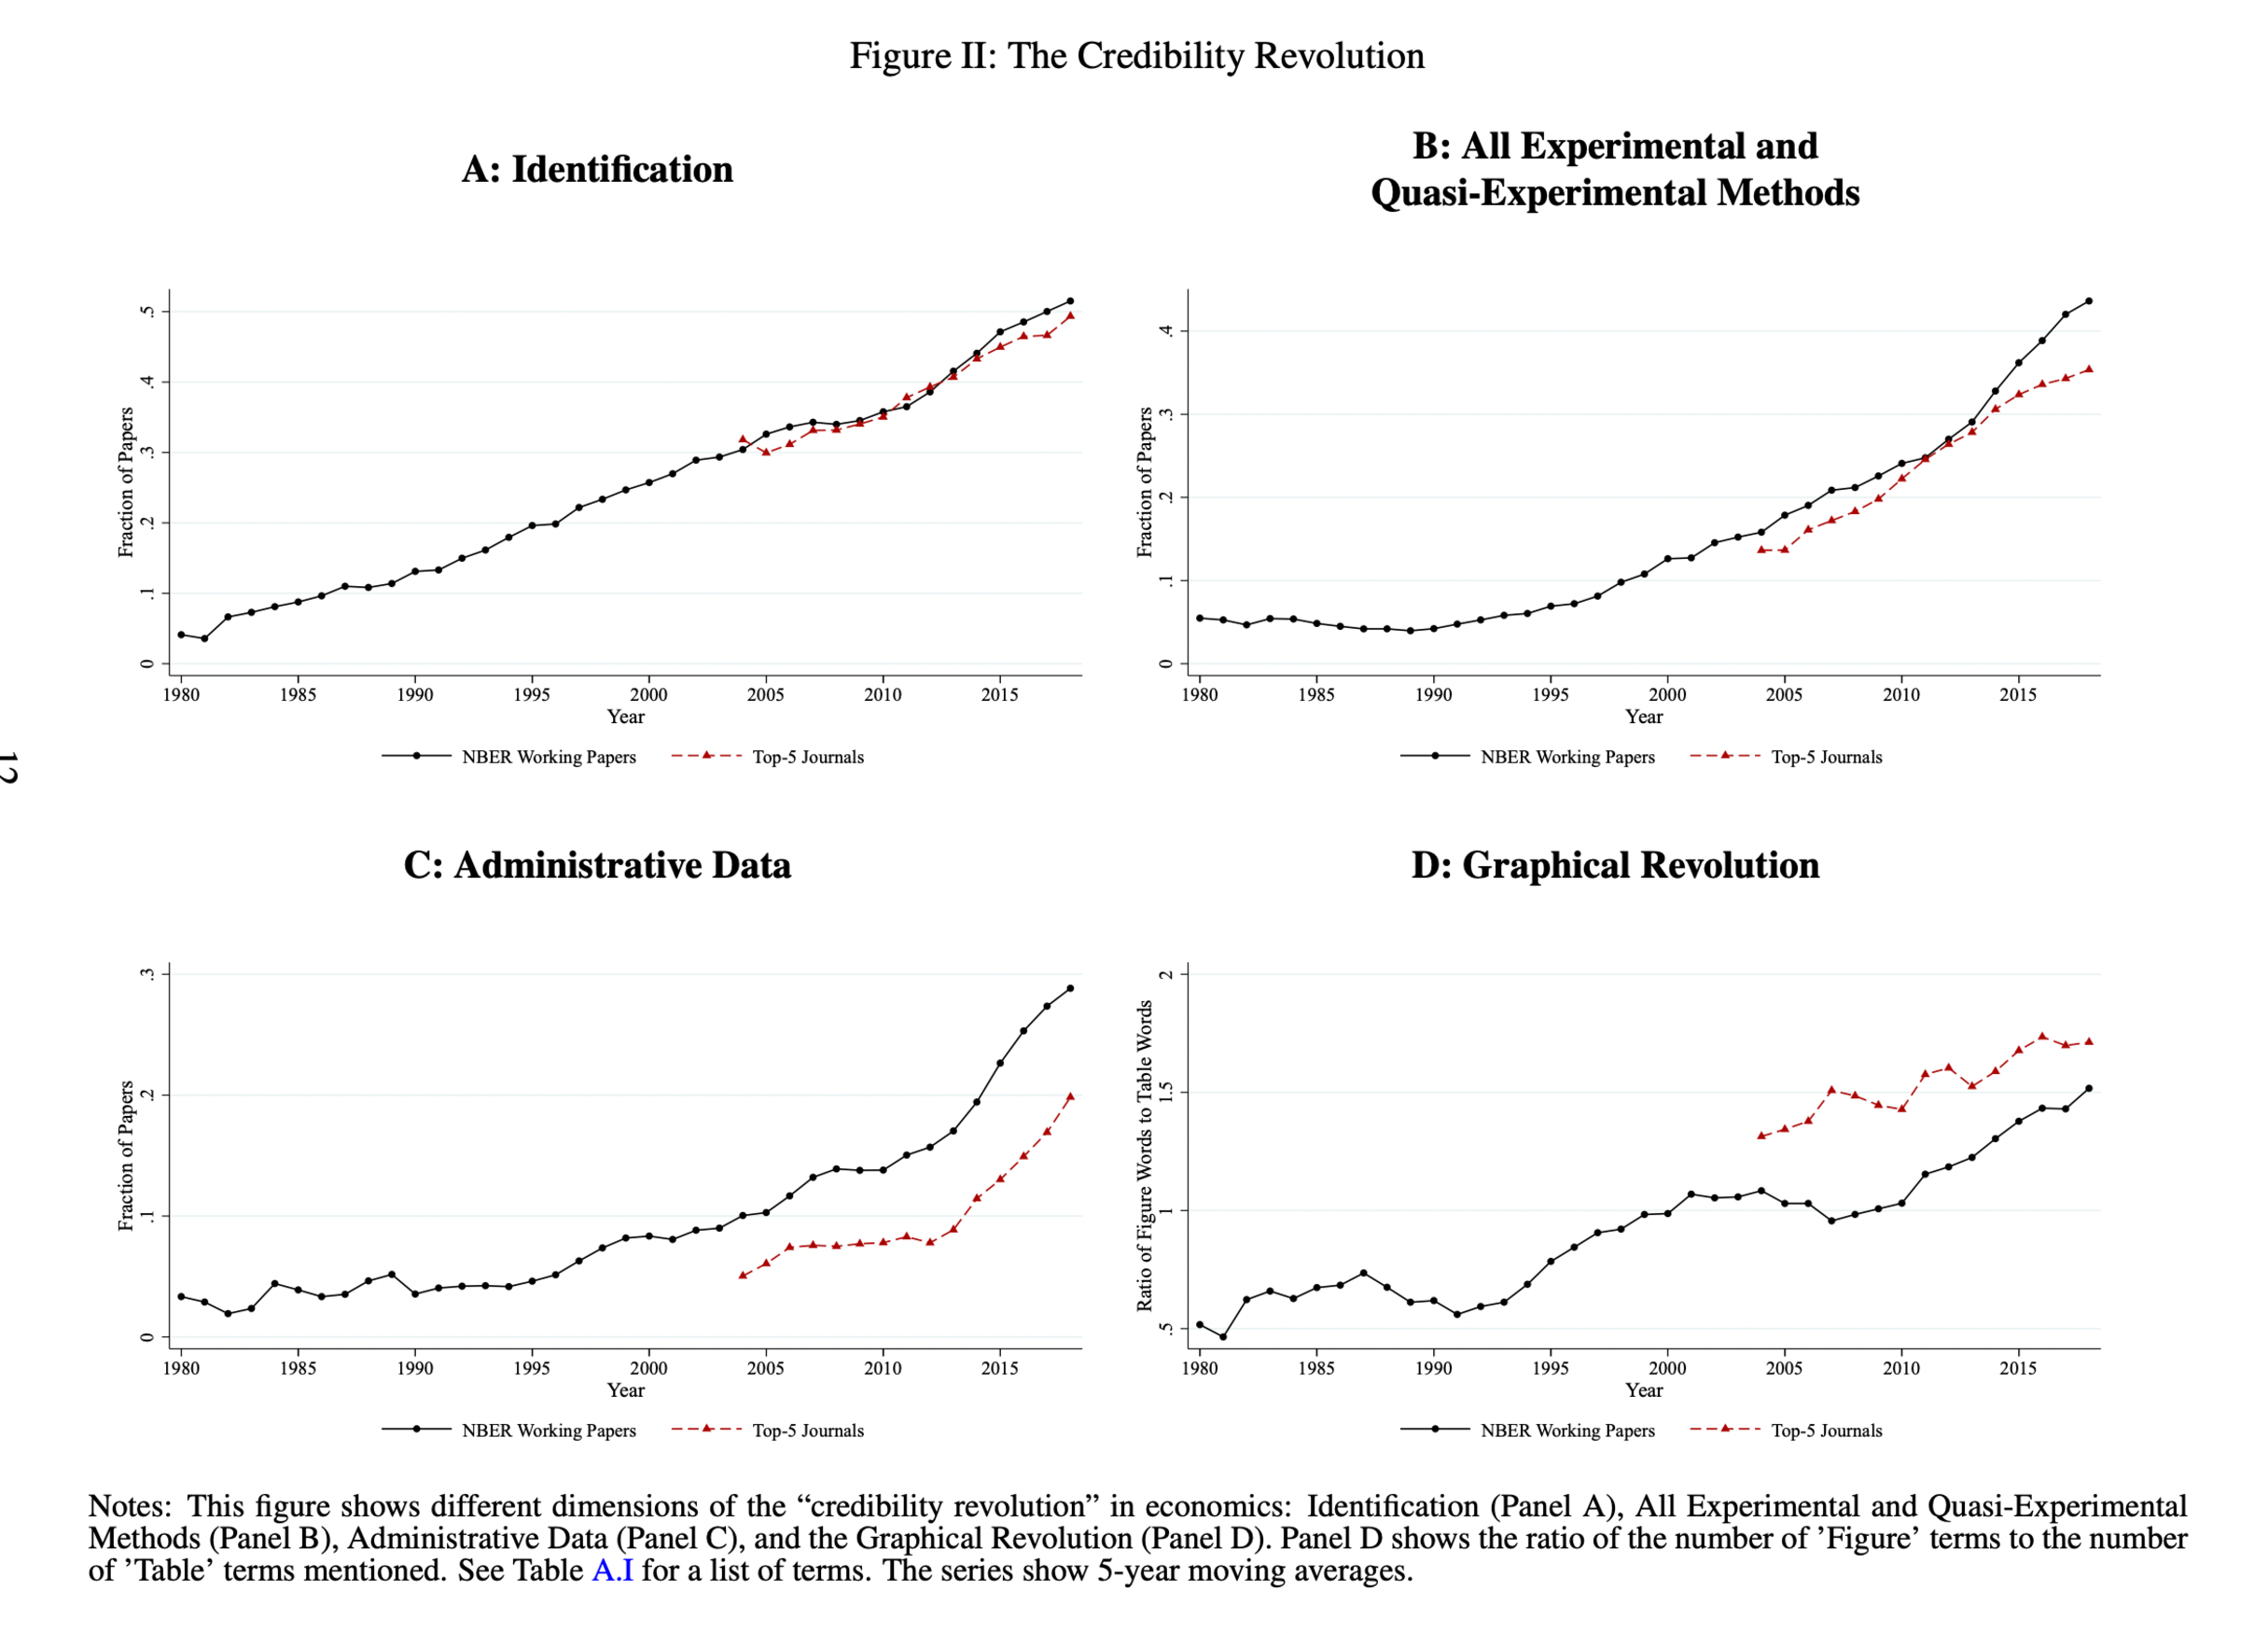
\includegraphics[width=1\textwidth]{kleven2}
\end{figure}
\end{frame}
\begin{frame}
\frametitle{Why is this course important?}
\begin{figure}[htb]
\centering
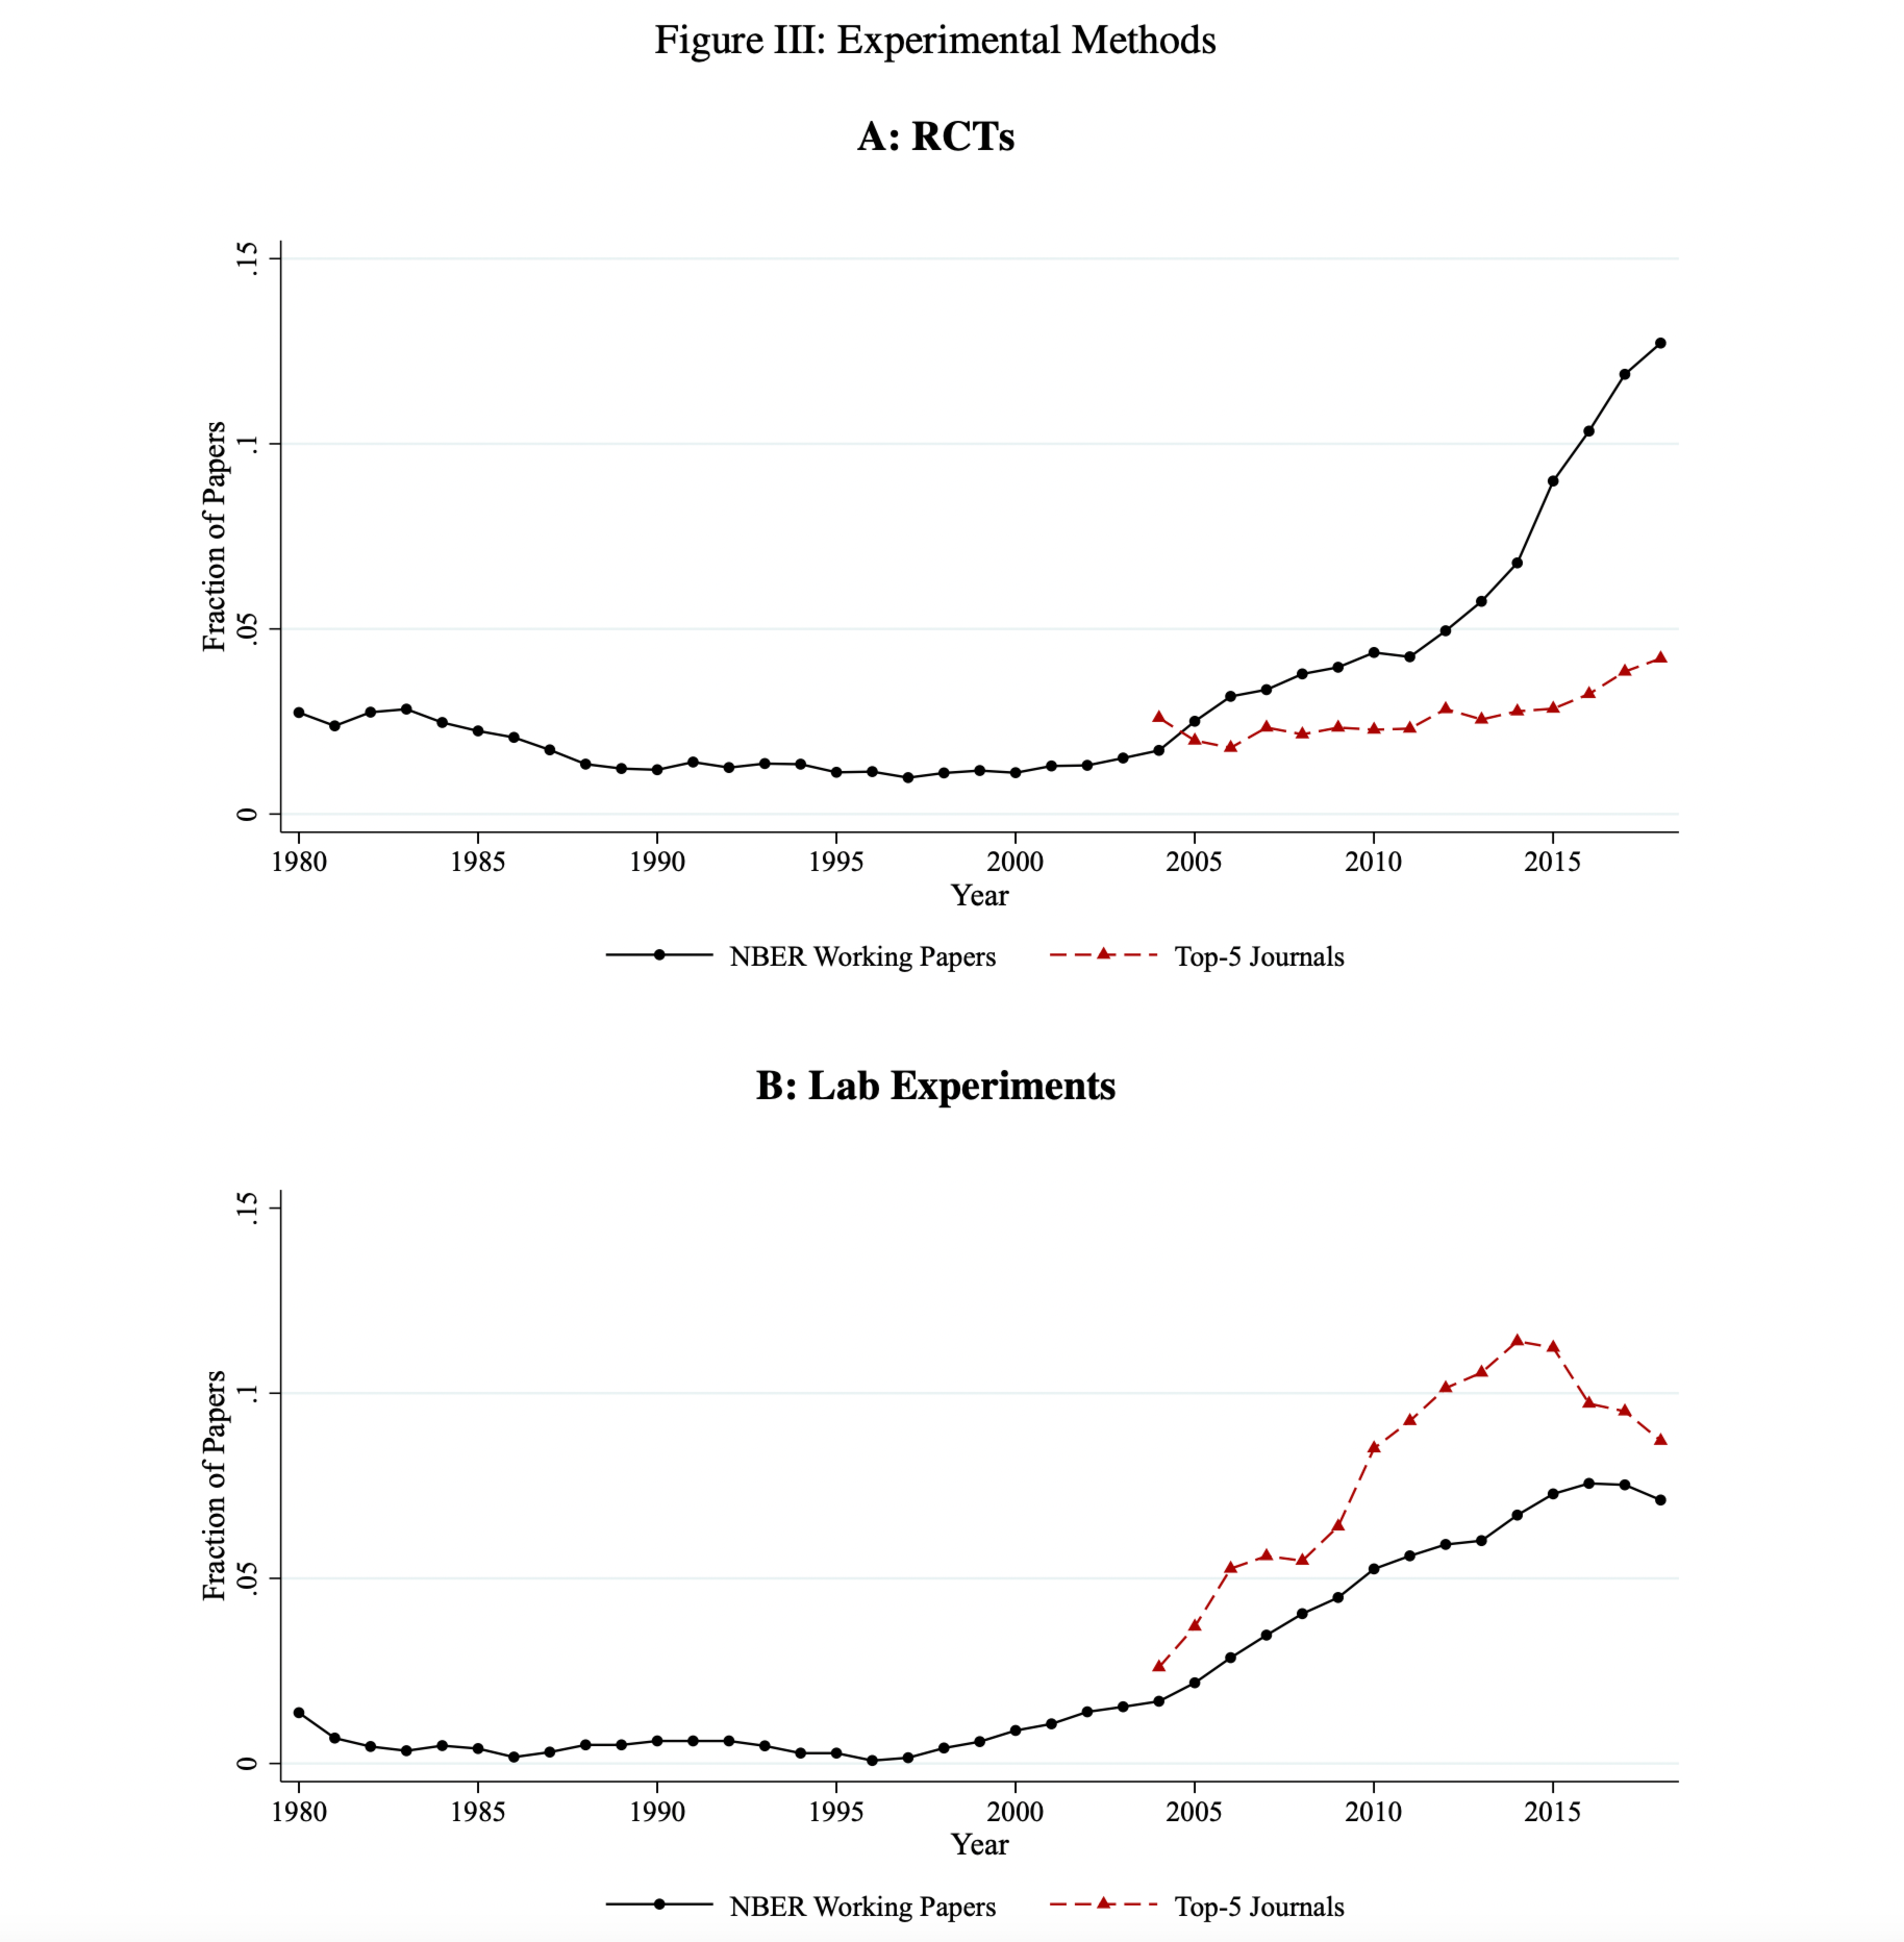
\includegraphics[width=1.1\textwidth]{kleven4}
\end{figure}
\end{frame}
\begin{frame}
\frametitle{Why is this course important?}
\begin{figure}[htb]
\centering
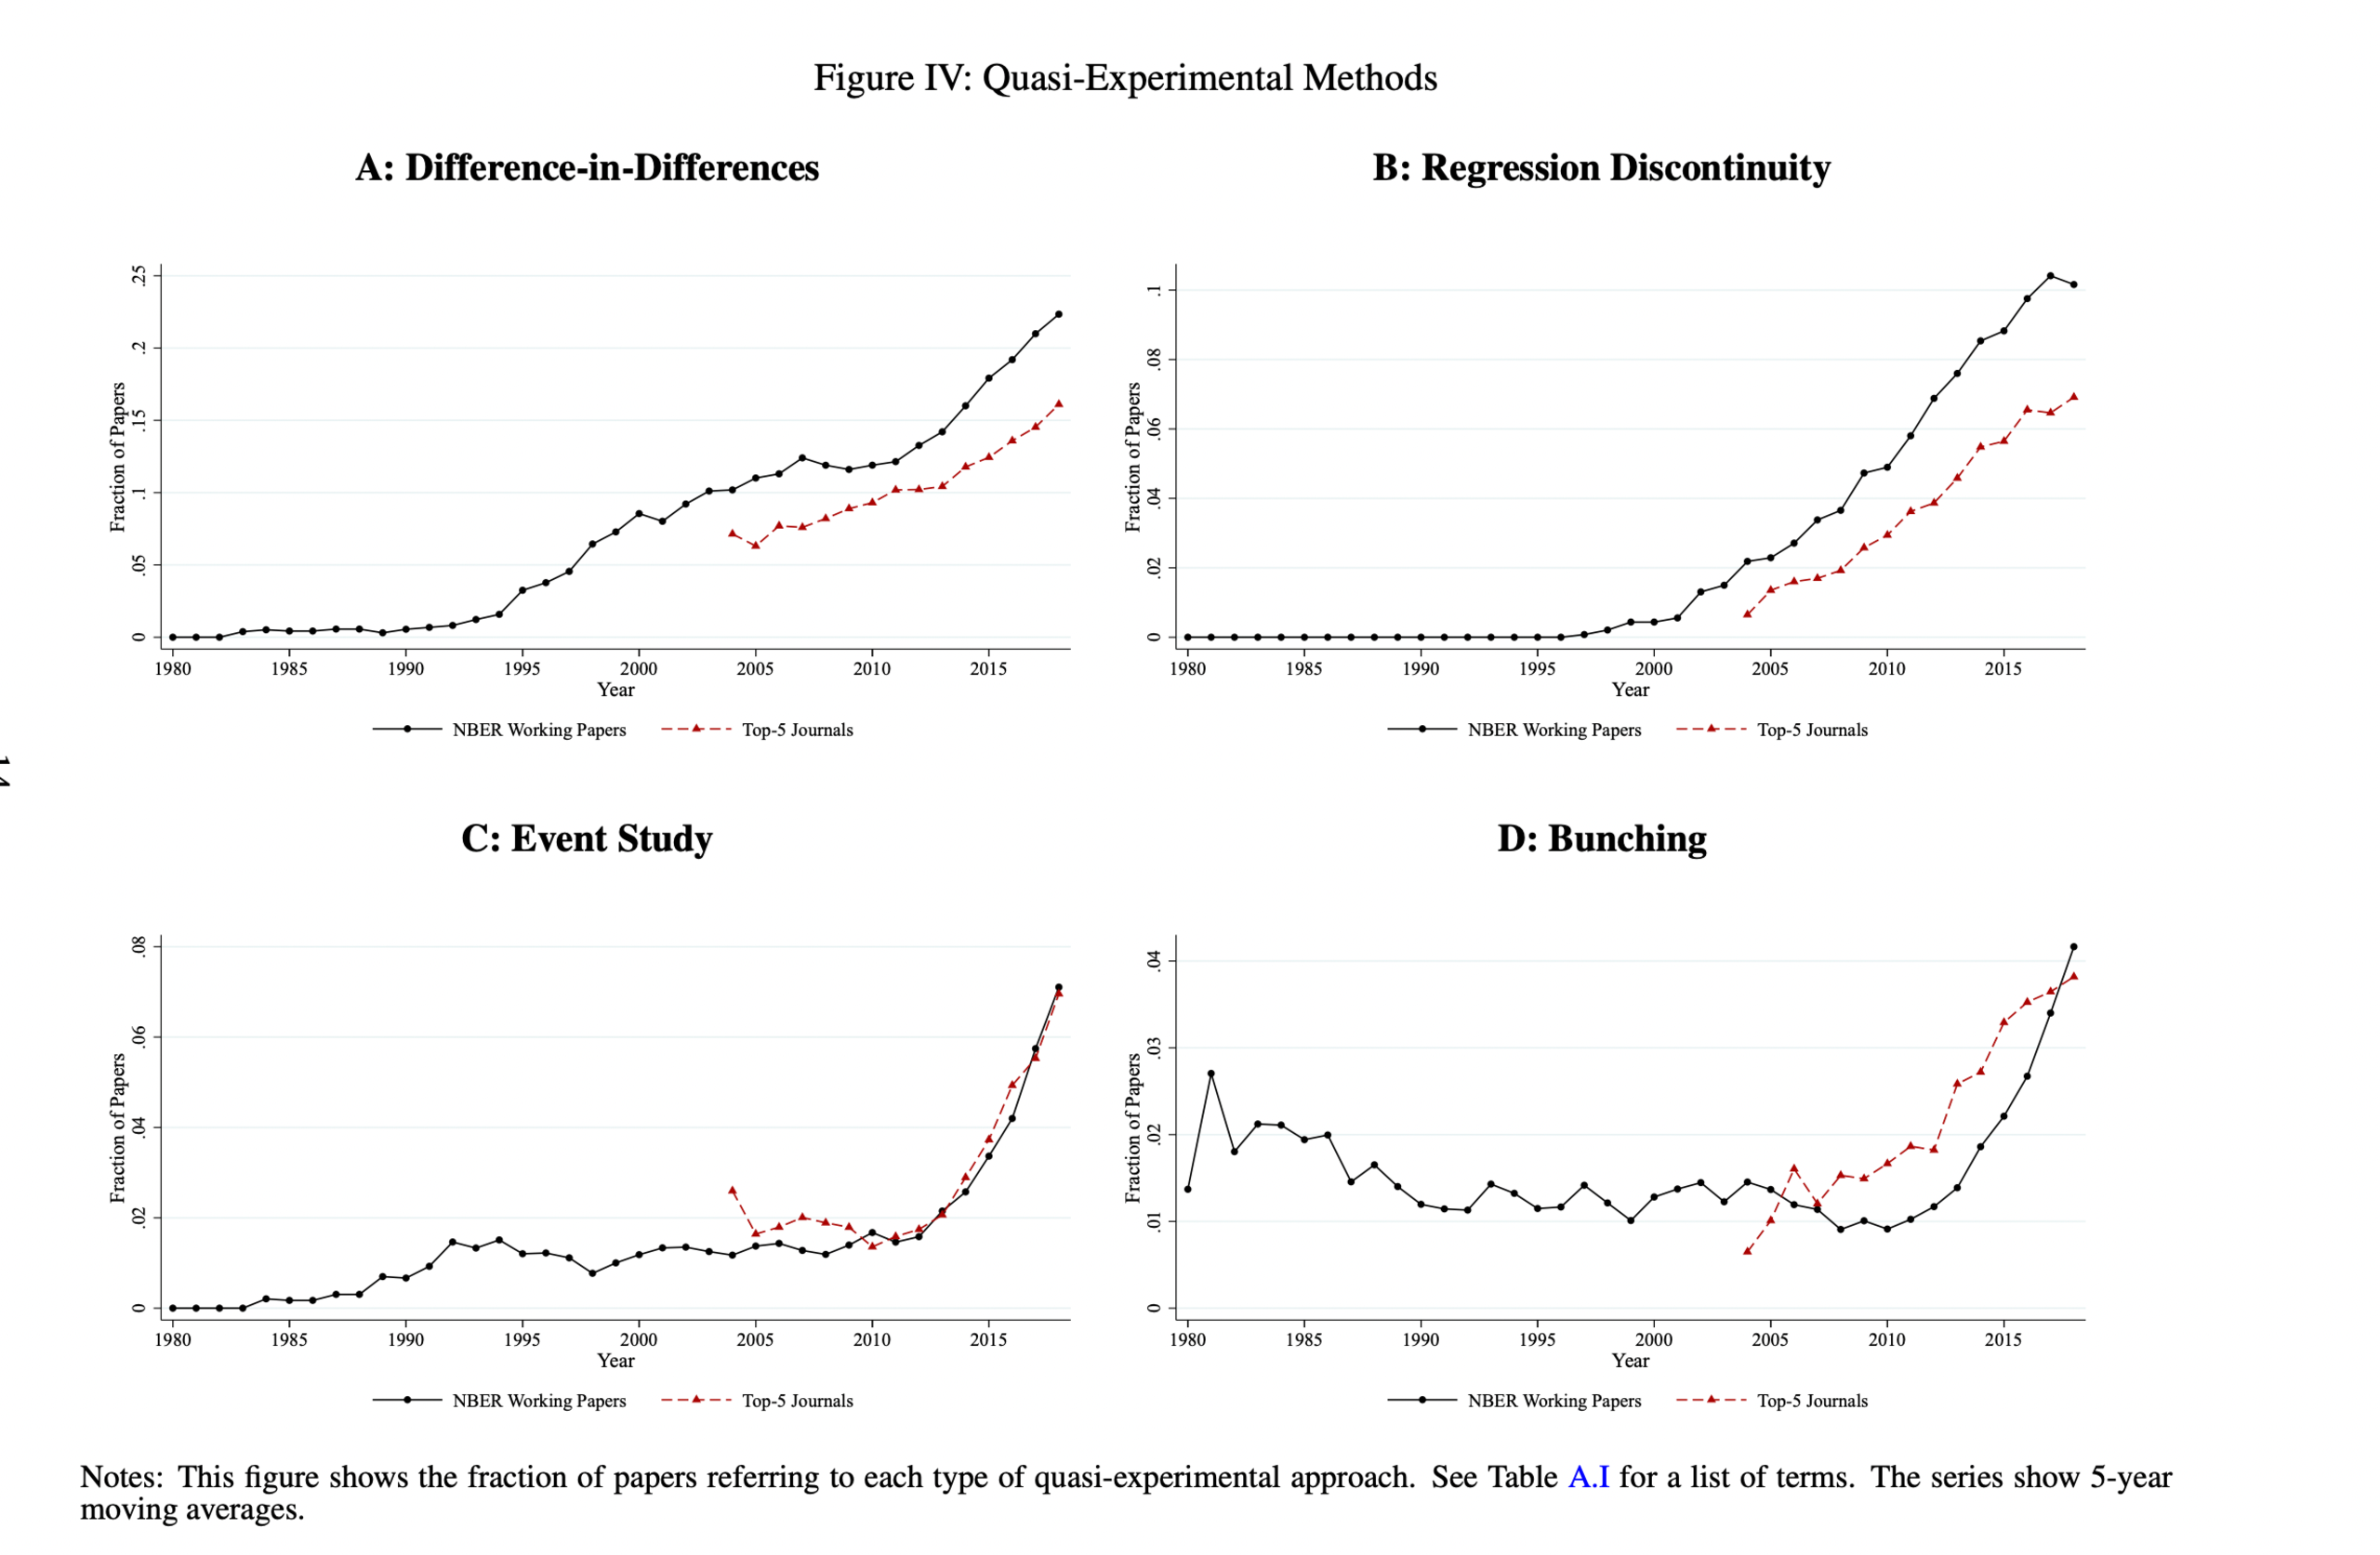
\includegraphics[width=1\textwidth]{kleven3}
\end{figure}
\end{frame}
%%
\begin{frame}
\frametitle{Economics is becoming more and more empirical, but... }
\begin{itemize}
\pause
\item But empirical work is hard
\begin{itemize}
\item Fundamentally messy.  
\item No clear start (statement of a theorem) and end (proof of the theorem).
\item Data is always messy $\rightarrow$ discretion will always come into play.
\item There is no Q.E.D at the end of empirical papers.
\end{itemize}
\bigskip
\pause
This can be overwhelming for grad students entering their third year.
\begin{itemize}
\item They need to do research \textit{independently}.
\item Often this research is empirical.
\item But most of your prior training was just about proving theorems...
\end{itemize}
\bigskip
Econ 628 is designed to smooth this transition (but this is hard for me too so feedback is very important!).  
\end{itemize}
\end{frame}
%%%%%%%%%%%%
\begin{frame}
\frametitle{Pop-Quiz! From Dynarski et al. (2021, AER)}
\pause

\includegraphics[width=0.8\textwidth]{aux/susan_abs}
\end{frame}
\begin{frame}
\frametitle{Pop-Quiz! From Dynarski et al. (2021, AER)}
\pause
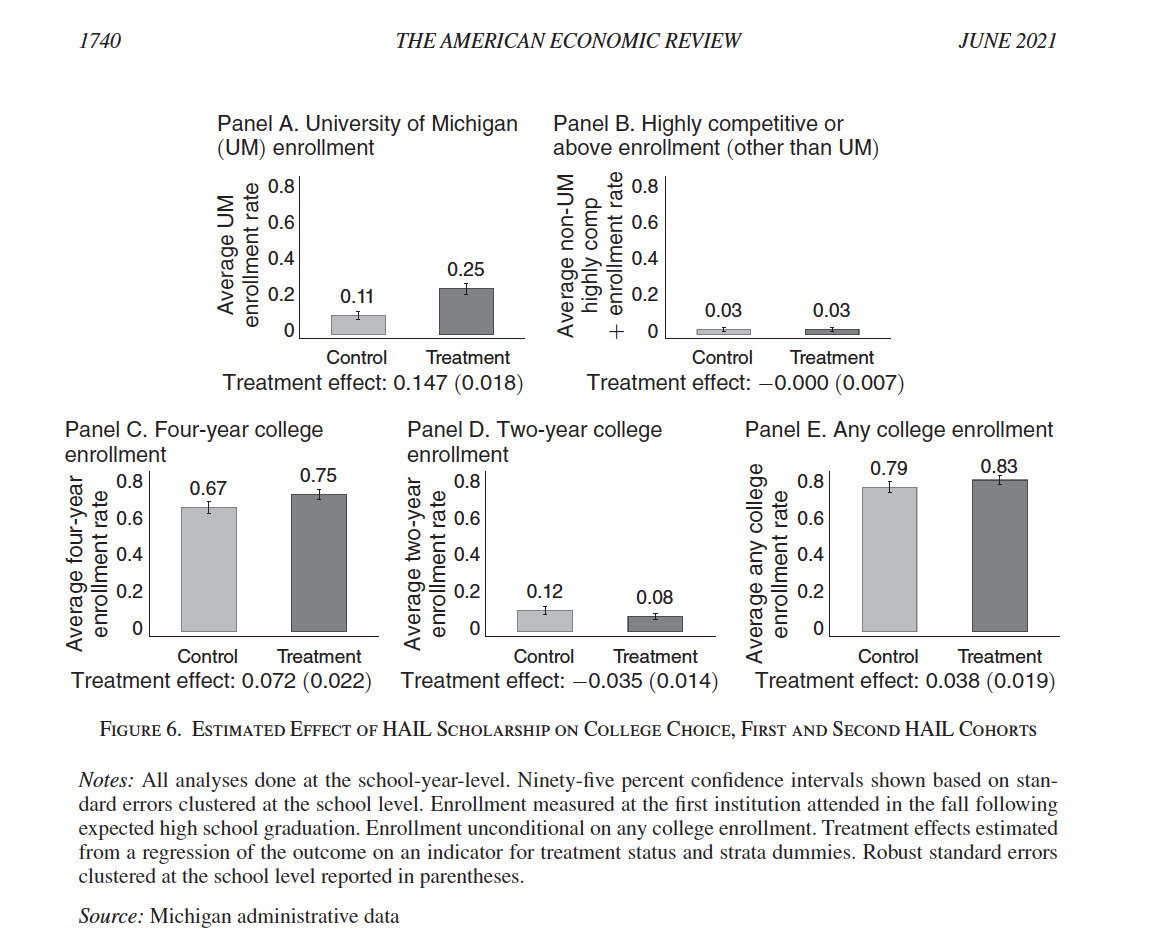
\includegraphics[width=0.8\textwidth]{aux/susan}
\end{frame}
%%
\begin{frame}
\frametitle{One more... (this is from MHE)}
\pause
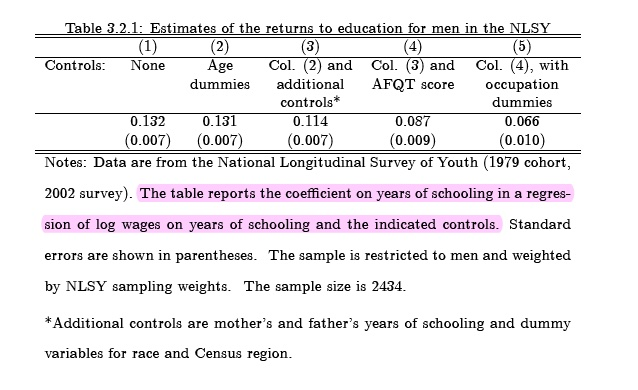
\includegraphics[width=0.8\textwidth]{aux/angrist_reg}
\end{frame}
\begin{frame}
\frametitle{Last one... (this is from Borjas, 1980)}
\pause
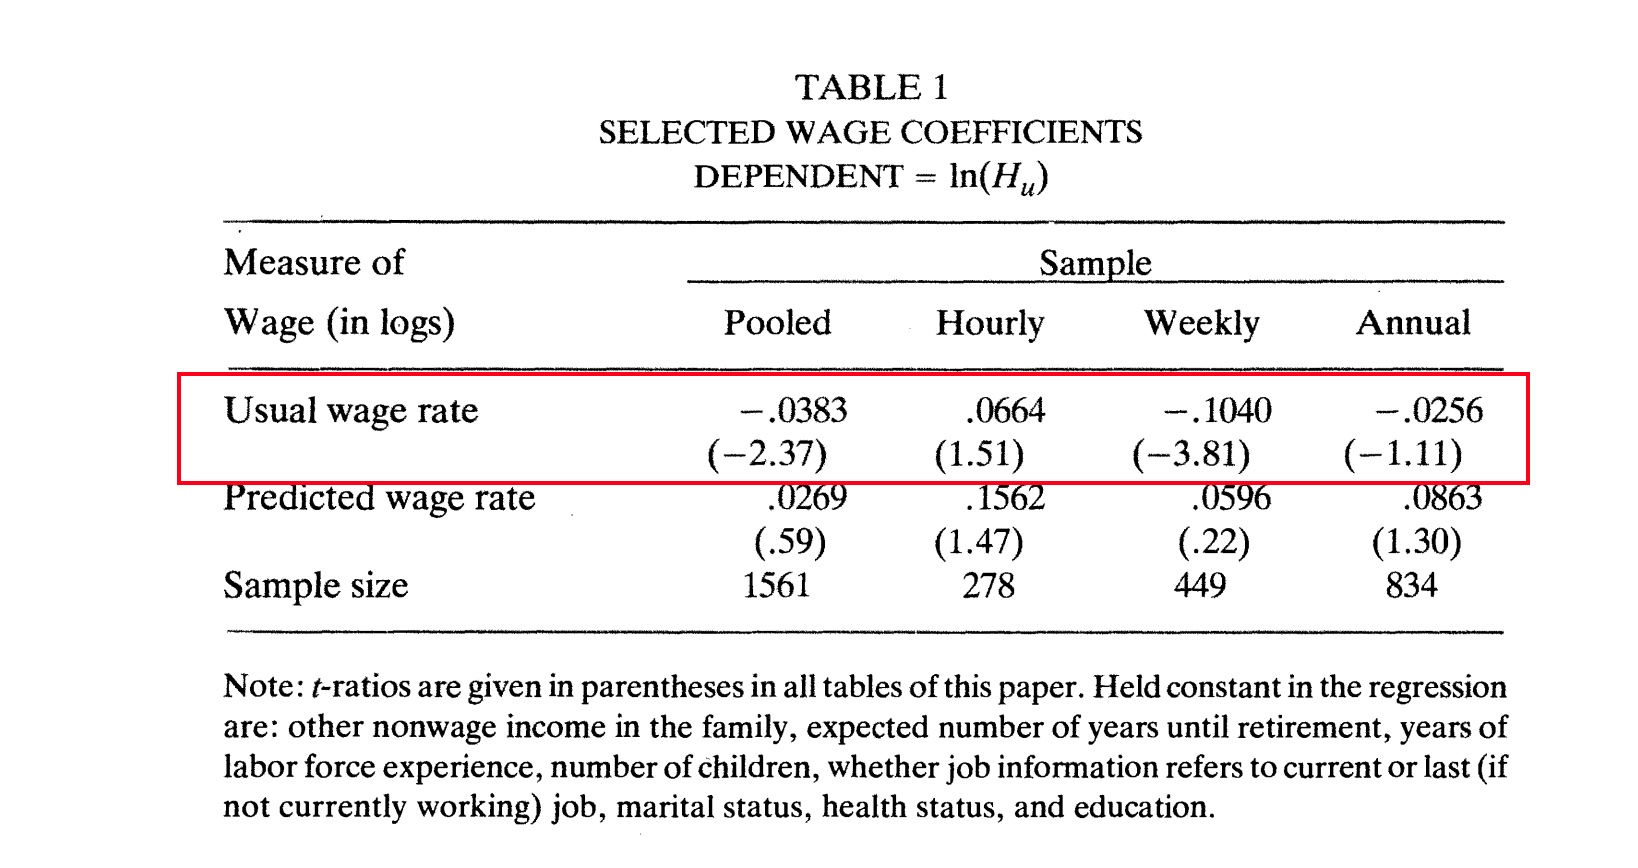
\includegraphics[width=0.8\textwidth]{aux/borjas}
\end{frame}



\begin{frame}
\frametitle{What is econometrics?}
\begin{enumerate}
\item Identification
\bigskip
\bigskip
\item Estimation
\bigskip
\bigskip
\item Inference 
\end{enumerate}
\end{frame}
%%
\begin{frame}
\frametitle{What is econometrics?}
\begin{enumerate}
\item Identification (What can be learned?)
\bigskip
\bigskip
\item Estimation (How do I learn it?)
\bigskip
\bigskip
\item Inference  (How certain should I be?)
\end{enumerate}
\pause
\bigskip
\begin{itemize}
\item Econometricians: new results in these areas.
\pause
\bigskip
\item Applied Economists: formulate hypothesis, apply tools 1-3 created by econometricians to real data.  
\end{itemize}
\end{frame}
%%
\begin{frame}
\frametitle{Why econometrics is not called statistics?}
\pause
\begin{itemize}
\item Good question. Some differences:
\bigskip

\begin{itemize}
\pause
\medskip
\item Applications to economic questions / data.
\medskip
\item Emphasis on causal relationship using observational data.
\medskip
\item Impose restrictions from economic theory.
\medskip
\item Emphasis on welfare and counterfactual distributions.
\end{itemize}
\end{itemize}
\end{frame}
\begin{frame}
\frametitle{Roadmap}
\begin{itemize}
\item Today: Establish a link between basic concepts in econometric models and their relationship with modern  notions of causality.
\bigskip
\item For a long time in economics causality could be achieved/discussed only \textit{after} having specified an econometric model.
\bigskip
\item An econometric model must have two fundamental features:
\medskip
\begin{itemize}
\item It tells us how the observed data were generated.
\medskip
\item It tells us how things would have been if we were to exogenously change one factor \textit{ceteris paribus}
\end{itemize}
\medskip
\item Econometric models impose structure on the data generating process (DGP)
\medskip
\item Knowledge of the DGP yields a probability measure $\mathbf{P}(.)$ over
the observed data $\mathbf{Y}$.
\end{itemize}
\end{frame}
%%%%

\begin{frame}
\frametitle{Taxonomy}
\begin{enumerate}
\item Parametric models: models are indexed by a finite dimensional vector of parameters.
\bigskip
\item Non-parametric models: models are indexed by infinite dimensional parameters (e.g. an unknown function).
\bigskip
\item Semi-parametric models: models are indexed by a finite dimensional vector parameters and an infinite dimensional nuisance function.
\end{enumerate}
\end{frame}
%%
\begin{frame}[shrink=2]
\frametitle{A parametric model}

\be
Y_{i} = \beta_{0} + \beta_{1}X_{i} + \varepsilon_{i}
\ee
\be
(X_{i},\varepsilon_{i}) \sim_{\text{iid}} \mathcal{N}\left[\left(\begin{array}{c}\mu \\0\end{array}\right),\left(\begin{array}{cc}\sigma^{2}_{x} & 0 \\0 & \sigma^{2}\end{array}\right) \right]
\ee
\be
\theta = (\beta_{0},\beta_{1},\mu,\log\sigma_{x},
\log\sigma)\in\mathcal{R}^{5}
\ee
\bigskip
\begin{itemize}
\item Everything there is to know about the world in 5 parameters.
\end{itemize}
\end{frame}
%%
%%
\begin{frame}[shrink=2]
\frametitle{A semi-parametric model}
\be
Y_{i} = \beta X_{i} + \varepsilon_{i}
\ee
\be
\E[\varepsilon_{i}\vert X_{i}]=0
\ee
\be
\beta\in\mathcal{R}
\ee
\bigskip
\pause
\begin{itemize}
\item Unrestricted distribution of $F_{X}(.)$ of $X_{i}$.
\item Mean restriction on conditional distribution of $F_{\varepsilon\vert X}$
\item Both objects potentially infinite dimensional (but nuisance?)
\end{itemize}
\end{frame}
%%
%%
\begin{frame}[shrink=2]
\frametitle{A non-parametric model}
\be
Y_{i} = g(X_{i},\varepsilon_{i})
\ee
\be
\varepsilon_{i} \bot X_{i} 
\ee
\be
g(.,.): \mathcal{R}^{2}\rightarrow[0;1] \text{  is monotone and increasing in both arguments}
\ee
\begin{itemize}
\item Unrestricted marginals of $\varepsilon$ and $X_{i}$.
\item Interested in function $g(.,.)$ or features such as $\E_{\varepsilon}[g(X_{i},\varepsilon_{i})]$.
\end{itemize}
\end{frame}
%%
%%
\begin{frame}
\frametitle{Identification}
\begin{itemize}
\item Identification is the study of which DGPs in the model space
can be ruled out given the joint distribution of observables.
\medskip
\item This question is asked in world where DGPs can be estimated infinitely many times (that is never confuse identification with estimation).
\medskip
\item Logical first step for any empirical project.
\medskip
\item If nothing is identified, not worth going into step 2 and 3 (estimation, inference).
\end{itemize}
\end{frame}
%%
\begin{frame}
\frametitle{Setup}
\begin{itemize}
\item Most models can be written as
\be
\mathbf{Y}_{i} = \mathbf{g}(\mathbf{U}_{i}), \qquad \mathbf{U}_{i}\sim_{iid}F_{U}(\mathbf{u})
\ee
\medskip
\item We call $\theta\equiv(\mathbf{g}(\mathbf{U_{i}}),F_{U})$ the structure of the model. 
\medskip
\item $F_{Y}(\mathbf{y})$ the distribution function governing the observed variables.
\medskip
\item $F_{\theta}(\mathbf{y})$ the distribution function implied by $\theta$ under the model.
\pause
\bigskip
\bigskip
\item Two structures $\theta'$ and $\theta''$ are observationally equivalent  if $F_{\theta'}(.) = F_{\theta''}(.)$
\end{itemize}
\end{frame}
%%
%%
\begin{frame}
\frametitle{Identification}
\begin{itemize}
\item The identified set is given by 
\be
\Omega(F_{Y},\Theta)=\{\theta \in \Theta: F_{\theta}(.) = F_{Y}(.)\}
\ee
\medskip
\item Structure is point identified is $\Omega(F_{Y},\Theta)$ is a singleton. 
\end{itemize}
\end{frame}
%%
\begin{frame}[plain]{Example: A Mixture Model}

Consider the model
\[
Y_{i}=\left(1+D_{i}\right)\varepsilon_{i},\mbox{ }\left(D_{i},\varepsilon_{i}\right)\overset{iid}{\sim}Bernoulli(p)\times N\left(0,1\right),\mbox{ }p\in\left(0,1\right)
\]

where we observe data on $Y_{i}$.

\pause{\bigskip{}
}
The parameter $p$ is point identified

\pause{\bigskip{}
}
\begin{proof}
By law of total probability:
\[
f_{Y}\left(y\right)=\phi\left(y\right)\left(1-p\right)+\frac{1}{2}\phi\left(\frac{y}{2}\right)p
\]
Solving for $p$, we have $p=\frac{f_{Y}\left(y\right)-\phi\left(y\right)}{\frac{1}{2}\phi\left(\frac{y}{2}\right)-\phi\left(y\right)}$
\end{proof}
\end{frame}
%%
%%
\begin{frame}[plain]{Over-id tests}

\begin{itemize}
\item How many moments in the data can help you identify $p$?
\be
p=\frac{f_{Y}\left(y\right)-\phi\left(y\right)}{\frac{1}{2}\phi\left(\frac{y}{2}\right)-\phi\left(y\right)}
\ee
\pause
\item Many!
\pause
\bigskip
\item Take the model seriously, does the above equation holds over the entire support of $y$?
\pause
\bigskip
\item This question is the foundation of over-identification tests. We will go back to this concept many times!
\end{itemize}
\end{frame}

\begin{frame}[plain]{Counterfactuals and Causality}

\begin{itemize}
\item Econometric models posit well defined \emph{counterfactuals} 
\end{itemize}

\pause{\bigskip{}
}
\begin{itemize}
\item Example:
\[
Y_{i}=f\left(X_{i},U_{i};\phi\right)
\]
\end{itemize}

\pause{\bigskip{}
}
\begin{itemize}
\item Causal effect of changing $X_{i}$ from $x'$ to $x''$:
\[
\Delta_{i}\left(x'',x'\right)\equiv f\left(x'',U_{i};\phi\right)-f\left(x',U_{i};\phi\right)
\]
\end{itemize}

\pause{\bigskip{}
}
\begin{itemize}
\item Need to be careful: can we change $X_{i}$ holding $f\left(.,.\right)$
and $U_{i}$ constant?
\medskip
\item More generally, what if my model is wrong? 
\end{itemize}
\end{frame}

\begin{frame}[plain]{Potential Outcomes}

\begin{itemize}
\item Statistics approach (Neyman-Rubin): Define counterfactuals ``atheoretically''
relative to what would emerge from an experiment.
\item Potential outcome $Y_{i}^{d}\equiv Y_{i}\left(d\right)$ gives what
results when unit $i$ is experimentally exposed to treatment $d$
\end{itemize}

\pause{\bigskip{}
}
\begin{itemize}
\item Example: Drug trial

\begin{itemize}
\item $D_{i}$: 1 if treated, 0 if placebo
\item $Y_{i}^{1}$: life span if treated
\item $Y_{i}^{0}$: life span if placebo
\end{itemize}

\pause{\bigskip{}
}
\item ``Fundamental problem of causal inference'' (Holland, 1986)
\[
Y_{i}=D_{i}Y_{i}^{1}+\left(1-D_{i}\right)Y_{i}^{0}
\]
\end{itemize}
\end{frame}

\begin{frame}[shrink=3]{Unconfoundedness and ATE}

\centering
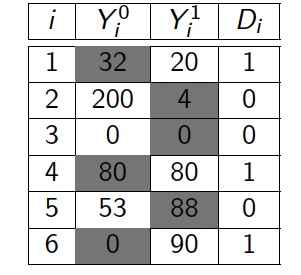
\includegraphics[width=0.3\textwidth]{aux/placebo}

\begin{itemize}
\item {\small{}Causal inference requires restrictions on the ``missing''
potential outcomes}{\small\par}
\item {\small{}Classic assumption: Unconfoundedness / Missing at Random
\begin{equation}
D_{i}\bot\left(Y_{i}^{1},Y_{i}^{0}\right)\mbox{ \ensuremath{\forall i}}\label{eq:MAR}
\end{equation}
}{\small\par}
\item Under the above assumption we can identify $ATE=\E[\Delta_{i}]=\E[Y_{i}^{1}-Y_{i}^{0}]$ 
\be
\begin{aligned}
\E[Y_{i}\vert D_{i}=1]-\E[Y_{i}\vert D_{i}=0] & =\E[Y_{i}^{1}\vert D_{i}=1]-\E[Y_{i}^{0}\vert D_{i}=0]  \\
& = \E[Y_{i}^{1}]-\E[Y_{i}^{0}] \\
& = \E[Y_{i}^{1}-Y_{i}^{0}] \\
& = ATE.
\end{aligned}
\ee
\end{itemize}
\end{frame}
%%
\begin{frame}[plain]{What would OLS identify?}
\begin{itemize}
\item We can express the potential outcome equation as follows
\be
\begin{aligned}
Y_{i} & =Y_{i}^{0}+(Y_{i}^{1}-Y_{i}^{0})D_{i} \\
& =\mu + \beta D_{i} + \varepsilon_{i}
\end{aligned}
\ee
where $\mu=\E[Y_{i}^{0}]$; $\beta= \E[Y_{i}^{1}-Y_{i}^{0}]$ and $\varepsilon_{i}=Y_{i}^{0}-\E[Y_{i}^{0}] + [(Y_{i}^{1}-Y_{i}^{0})-\E(Y_{i}^{1}-Y_{i}^{0})]D_{i}$
\pause
\bigskip
\item Does this look familiar?
\pause
\bigskip
\item Just run OLS and you will get back ATE since randomization ensures that $\E[D_{i}\varepsilon_{i}]=0$
\pause
\bigskip
\item Where is the randomness or uncertainty coming from here? 
\end{itemize}
\end{frame}
%%
\begin{frame}[plain]{Potential Outcomes vs Structural Models (Two Worlds)}

\begin{itemize}
\item ``Treatment effects'' literature relies on PO notation

\begin{itemize}
\item avoids restrictions on outcomes in favor of non-parametric restrictions
on assignment mechanism
\item emphasizes ``internal validity'' and impacts on observables
\end{itemize}

\pause{\medskip{}
}
\item ``Structural'' econometrics literature relies on latent variable
notation

\begin{itemize}
\item combines restrictions on outcomes with restrictions on assignment
\item emphasizes ``external validity'' and welfare impacts
\end{itemize}

\pause{\medskip{}
}
\item Less assumptions better but can't get something for nothing
\medskip
\item Important to consider implicit assumptions present in both approaches..
\medskip
\item Successful JMPs combine both approaches (complements, not substitutes!).
\end{itemize}
\end{frame}

\begin{frame}[plain]{SUTVA}

\begin{itemize}
\item When are potential outcomes well defined?
\item Rubin (1986): Stable Unit Treatment Value Assumption (SUTVA)


\pause{\medskip{}
}
\begin{itemize}
\item Homogeneity: doesn't matter \emph{how} you apply the treatment. 


\pause{\medskip{}
}
\item No interference between units: my outcome only depends on my treatment
status
\[
Y_{i}\left(d_{1},d_{2},...,d_{i},....,d_{N}\right)=Y_{i}\left(d_{i}\right)
\]
\end{itemize}
\end{itemize}

\pause{\medskip{}
}
\begin{itemize}
\item Note that these assumptions are typically embedded in the $f\left(.,.\right)$
of a structural model:
\[
Y_{i}=f\left(D_{i},\varepsilon_{i}\right)
\]
\end{itemize}
\end{frame}
%%%%%%%%
\begin{frame}[plain]{Which if's have causal answers?}
\begin{itemize}
\item Large literature (e.g., Oaxaca, 1978) attempts to infer racial/gender
discrimination from wage regressions
\item Q1: What is the effect of being black (as opposed to white) on wages?
\end{itemize}

\pause{\medskip{}
}
\begin{itemize}
\item Holland (1986): Q1 not well defined

\begin{itemize}
\item Race is an ``attribute'' not a ``treatment.'' Can't be changed
ceteris paribus.
\item ``No Causation Without Manipulation!''
\end{itemize}

\pause{\medskip{}
}
\item Q2: What is the effect of being perceived to be black (as opposed
to white) on wages?

\begin{itemize}
\item Perceptions can be manipulated (e.g. Bertrand and Mullianathan, 2004).
\item Explosion of ``Audit Studies" $\rightarrow$ Another thing ``invented" by Economists?
\end{itemize}
\end{itemize}
\end{frame}
\begin{frame}
\frametitle{Systematic Discrimination among US Employers}
\begin{figure}[htb]
\centering
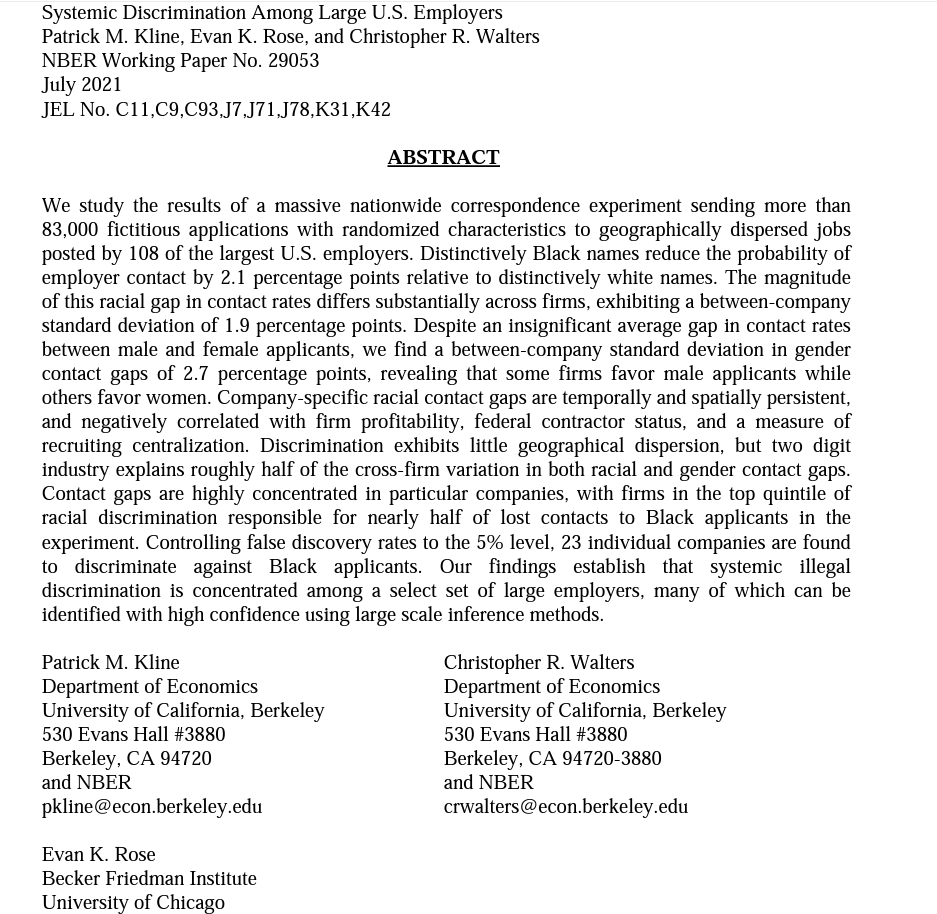
\includegraphics[width=1\textwidth]{aux/discriminate}
\end{figure}
\end{frame}
%%
\begin{frame}[plain]{Causal effects of choices}

\begin{itemize}
\item What is the causal effect of choices made by agents?
\item Q3: What is the effect of one extra year of education on earnings? What is the effect of going to private vs. public college? What is the effect of attending early childhood education programs? What is the effect of studying harder?
\end{itemize}

\pause{\medskip{}
}
\begin{itemize}
\item Very hard for an outsider (e.g. government) to directly manipulate these choices
\item Often ``we" can only encourage these choices.
\item Holland: can only talk about effect of encouragement. 
\end{itemize}

\pause{\medskip{}
}
\begin{itemize}
\item Does this invalidate most of econometrics?
\item tl;dr: No! We can impose structure to learn more (+ sometimes it is perfectly ok to only discuss effects of encouragement).
\item More on this when we'll talk about IV.
\end{itemize}
\end{frame}
%%%%%%%%
\end{document}

